%!TEX root = /Users/stevenmartell1/Documents/iSCAM-project/docs/iSCAM-guide/userGuide/usrGuide.tex
% 
% \section{Example: Simulation based on Strait of Georgia Pacific herring}
% \begin{multicols}{2}
% 
% \subsection{Introduction \& purpose}
% The purpose of this example is to demonstrate how to use \iscam\ to simulate data with known parameter values and then demonstrate the ability of the model to estimate the unknown parameters with and without observation and process errors.  This example is based on data from the Strait of Georgia Pacific herring fishery.
% 
% There are three distinct commercial fishing fleets for Pacific herring in the Strait of Georgia that have operated, and continue to operate, between 1951 and 2010 (Figure \ref{pHerringFig1}).  The first of these fleets is a purse seine fishery that generally operates in the winter months and historically used to catch herring for a reduction fishery and since the 1970s is now a much smaller bait fishery operation.  Since the early 1970s a much more valuable seine fishery for sac roe has been in operation along with a gill net fishery that also targets spawning female herring for its roe.
% 
% \begin{figurehere}
% 	% Requires \usepackage{graphicx}
% 	%\psfrag{Catch (t)}[][c]{Catch (1000 mt)}
% 	%\psfrag{Year}[][c]{Year}
% 	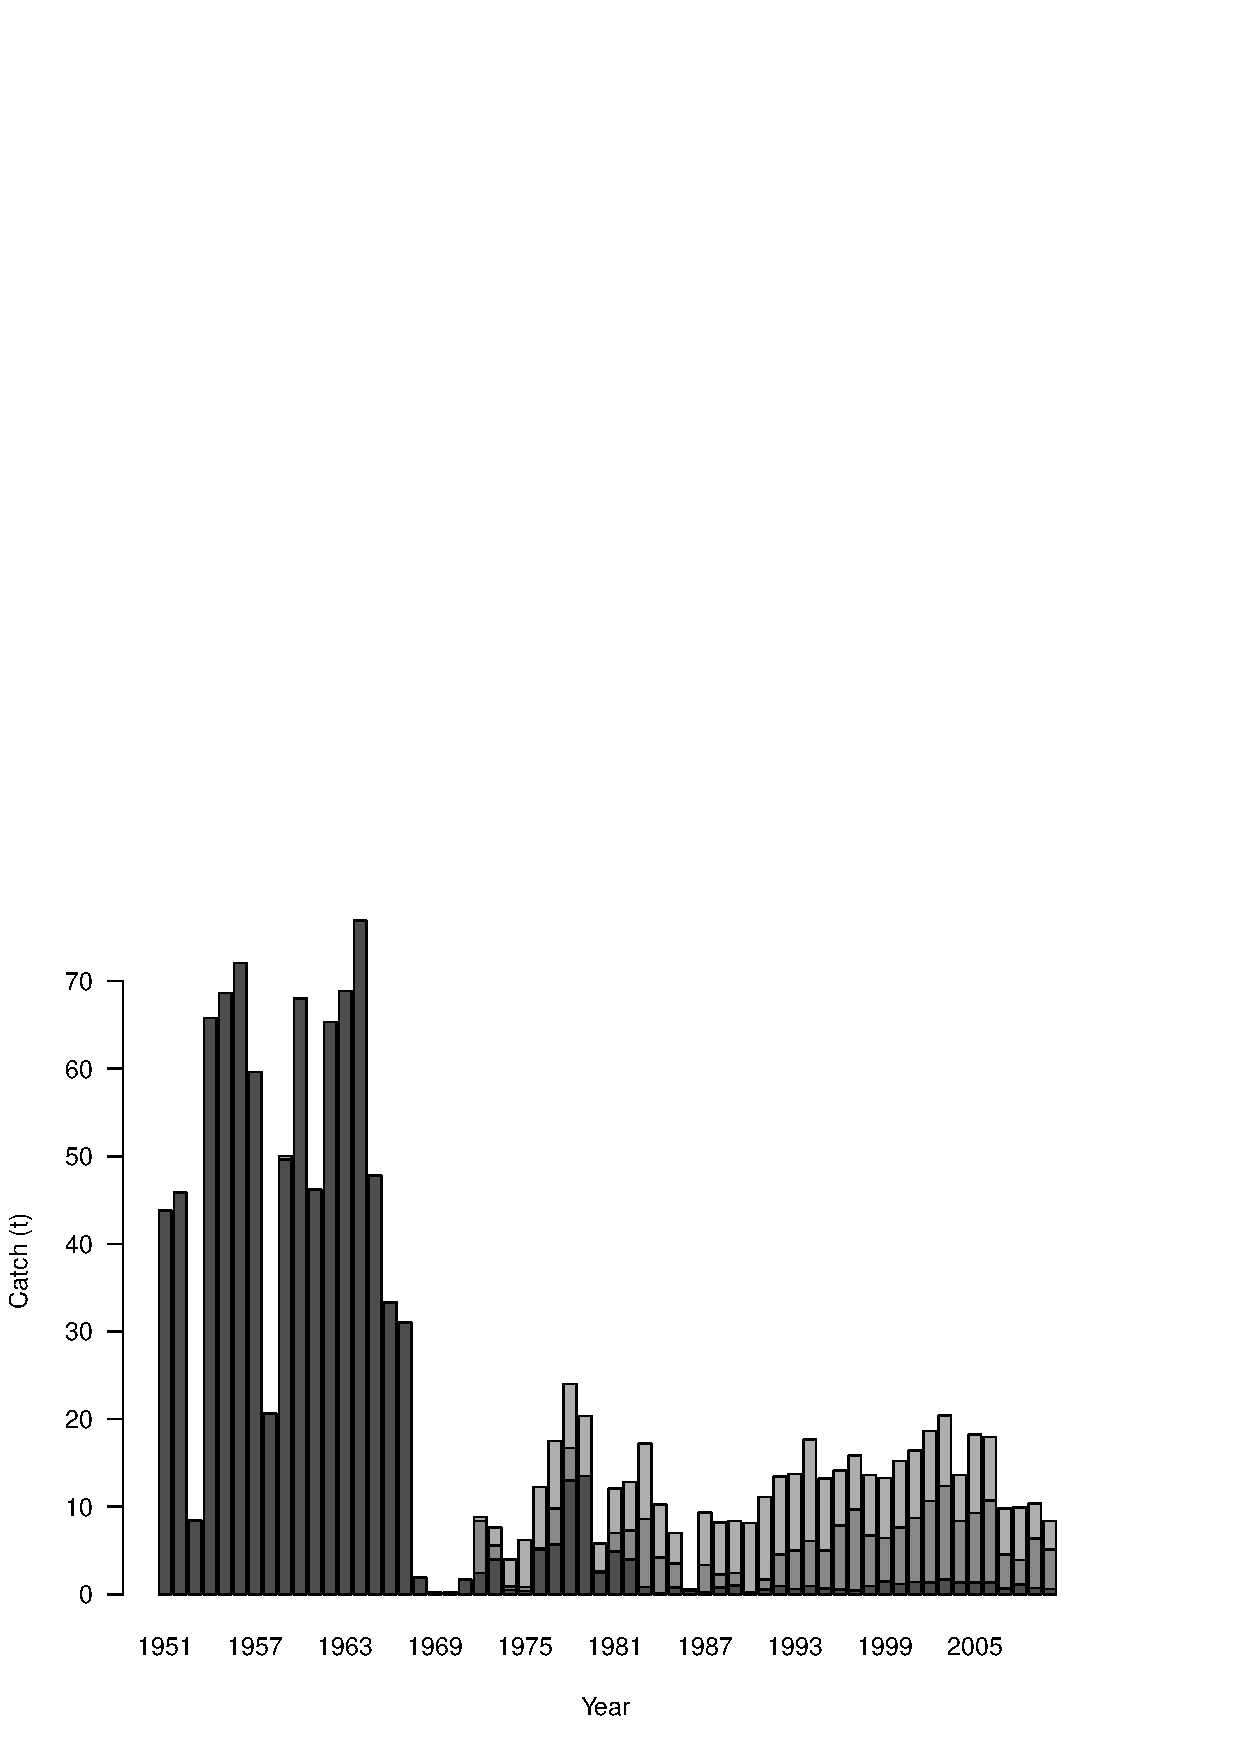
\includegraphics[width=\columnwidth]{iscamfigs/pHerringFig1.pdf}\\
% 	\caption{Total landings of Pacific herring in the Strait of Georgia stock assessment region by purse-seine (dark bars), Sn-roe (medium) and gill net (light bars).}\label{pHerringFig1}
% \end{figurehere}
% 
% 
% \subsection{Data \& control files}
% The available data for the herring fishery consist of commercial landings for each of the three fisheries, age-composition data from each of these fisheries (see Figure \ref{pHerringFig3} for the winter purse seine fishery), average weight-at-age of the catch, and a fisheries independent spawning biomass index (based on spawn deposition).  The spawn survey index is split into two separate series that correspond to a change in methods for estimating spawning deposition between 1987 and 1988.  The model is fit to all of these data and uses the empirical weight-at-age data to convert numbers-at-age to biomass.
% 
% 
% 
% 
% In this example, the command line option \texttt{-sim 000} is invoked to simulate fake data based on parameter values specified in the control file.  Recall the command line option \texttt{-sim} is used to tell \iscam\ to overwrite the existing observations in memory with simulated values (in this case with zero error because the random number seed is set to 000), and then attempt to estimate these model parameters.  If all is working correctly, the \texttt{iscam.par} file should have nearly identical estimates for the model parameters as the initial values that are specified in the control file.
% 
% The control file used in this example is shown here, and there are a couple of things that should be highlighted with simulating data with no error.  First off, the phase for the variance and variance partitioning parameters ($\vartheta$ and $\rho$, respectively) should be set to a negative value and not be estimated.  Second ensure that the upper bound for $\vartheta$ (vartheta or the total precision) is set to a very high value (say 5000) and the initial value is set close to the upper bound (4999 in this case).  The reason for fixing the parameters should be obvious, there is no error in the data to begin and thus its not necessary to estimate the total variance.  The reason to set the initial value of $\vartheta$ to a large value is to minimize the a slight bias due to the lognormal bias correction in the stock-recruitment relationship (i.e., the $-0.5\tau^2$ in \ref{T4.12} or \ref{T4.13}) during the parameter estimation phase.  If you do not specify a large value of $\vartheta$ then it is unlikely that you will obtain nearly exact estimates of the unfished recruitment $R_o$.
% 
% 
% %%Here is a pdf figure rotated.
% \begin{figurehere}
% 	% Requires \usepackage{graphicx}
% 	\centering
% 	%\psfrag{Year}[][c]{Year}
% 	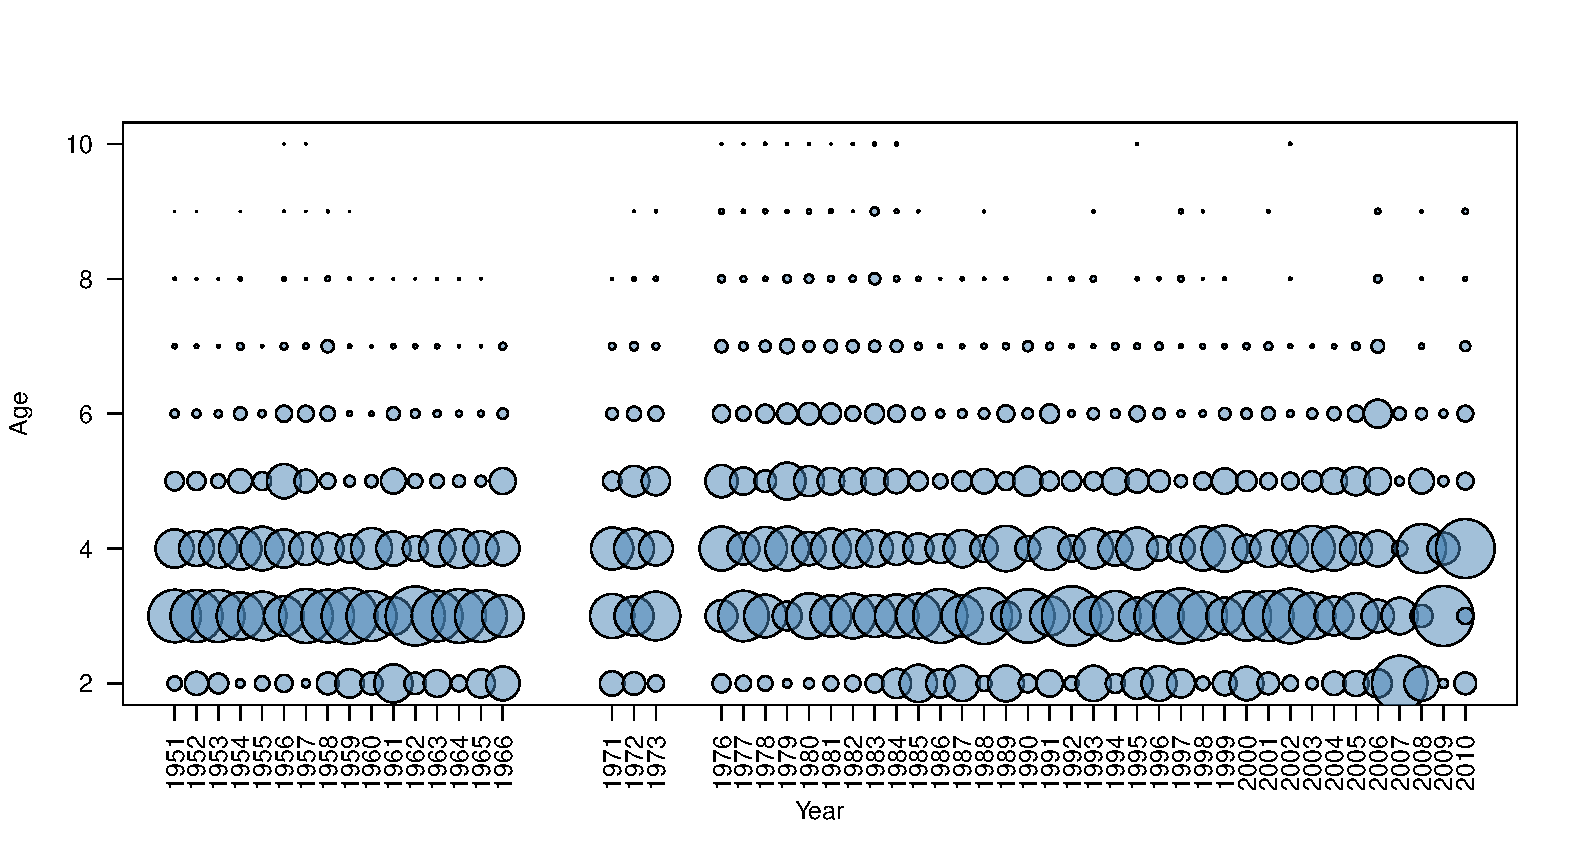
\includegraphics[height=\columnwidth,angle=-90]{iscamfigs/pHerringFig3.pdf}\\
% 	\caption{Age comps for the purse seine fishery in the Strait of Georgia between 1951 and 2010.}\label{pHerringFig3}
% \end{figurehere}
% \vspace{0.1in}
% 
% \noindent \hrulefill\\
% \small
% Control file for the SOG herring example
% \tiny
% \begin{alltt}
% \input{../../../Examples/sogHerring/SOGHerring2010sim.ctl}
% \end{alltt}
% \hrulefill
% \normalsize
% 
% 
% \subsection{Results}
% The ability of the model to estimate the parameters is demonstrated by the estimates of spawning stock biomass and the estimated fishing mortality rates for each of the fisheries.  Shown in Figure \ref{pHerringFig2} is the estimated pre-fishery biomass and the spawning stock biomass for the simulated data where the true values for the spawning stock biomass are shown by the filled circles.  Estimates of spawning stock biomass exactly match the true values that were used to simulate the data.  Departures from the true values when there is no simulated error would imply a structural problem, or potential coding error, and should be investigated further before proceeding with an actual assessment.
% 
% 
% \begin{figurehere}
% 	% Requires \usepackage{graphicx}
% 	\psfrag{Year}[][c]{Year}
% 	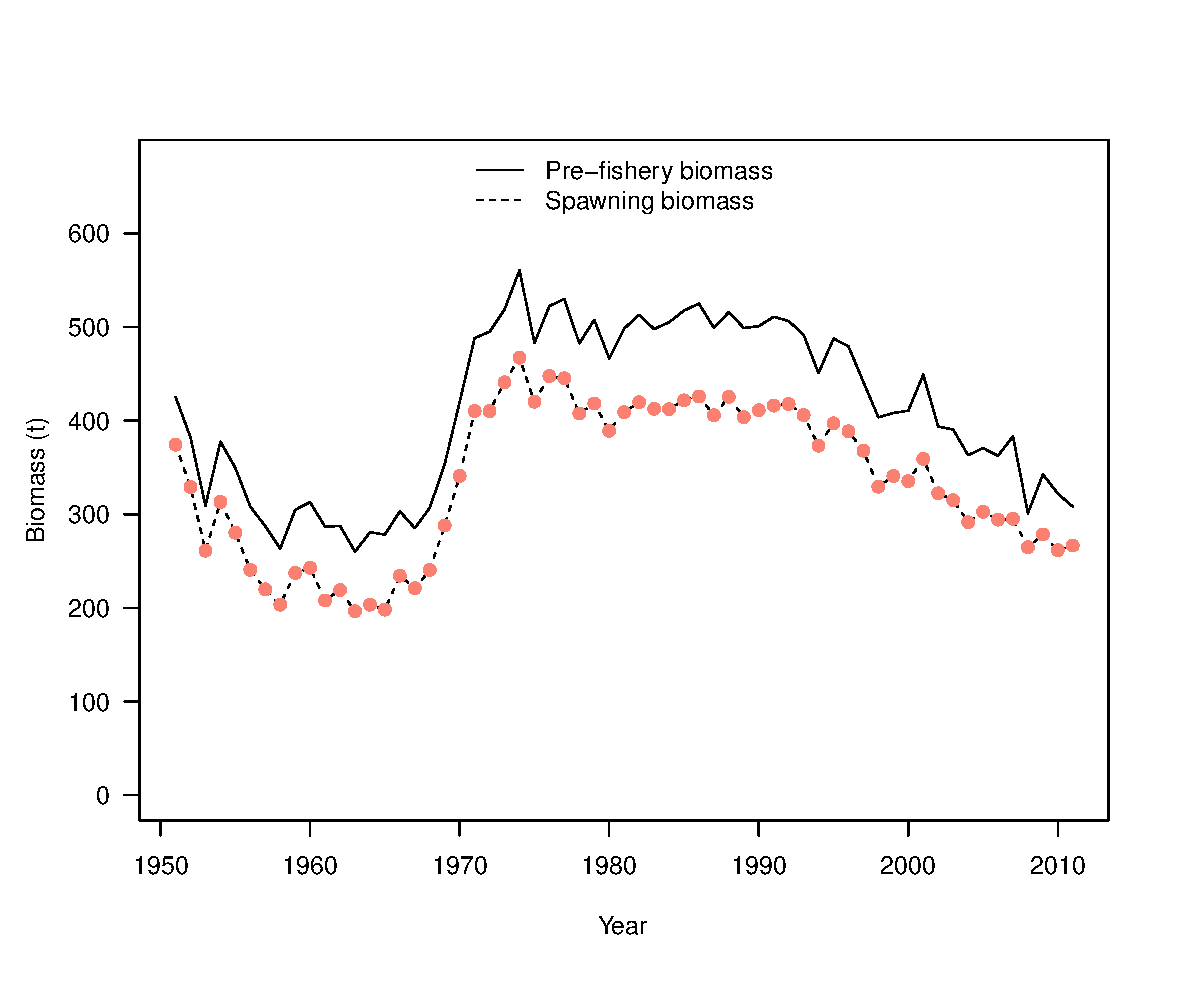
\includegraphics[width=\columnwidth]{iscamfigs/pHerringFig2.eps}\\
% 	\caption{Estimates of pre-fishery biomass and spawning stock biomass (lines) from \iscam\  in comparison to the true spawning stock biomass (filled points) based on the simulation model. No errors were generated in the simulation model.}\label{pHerringFig2}
% \end{figurehere}
% 
% 
% 
% \end{multicols}
% 




%%%%%%%%%%%%%%%%%%%%%%%%%%%%%%%%%%%%%%%%%%%%%%%%%%%%
%%%%%%%%%%%%%%%%%%%%%%%%%%%%%%%%%%%%%%%%%%%%%%%%%%%%
%%%%%%%%%%%%%%%%%%%%%%%%%%%%%%%%%%%%%%%%%%%%%%%%%%%%


\section{Example Assessment: the Namibian hake case study}
\begin{multicols}{2}
As a simple example of fitting \iscam\ to CPUE data only, we use the Namibian hake case study from chapter 10 in the Ecological Detective \citep{hilborn1997ecological}.  In this example the available data consist of catch (thousands of tons) and CPUE (tons per standardized trawl hour).  \cite{hilborn1997ecological} provide three alternative models to the data that range from simple 4 parameter Schaefer production models (observation \& process error only) and a 5 parameter lagged recruitment, growth/survival model.  In this example they assume the stock is at an unfished state in 1967.

To conduct the assessment using \iscam\ with the same unfished assumption in 1965, the 			``Assume unfished in first year (0=FALSE, 1=TRUE)'' flag must be set to 1 (see the following control file). \iscam\ is an age-structured model, and in this example there are no available age-composition data to compare with. Therefore we must also assume a selectivity curve for this fishery.  In this example, selectivity was assume to follow a logistic function with the 50\% vulnerability-at-age equal to 3.5 years with a standard deviation of  1.0 years.  It is also necessary in this case to turn off the estimation of the selectivity parameters by setting the estimation phase to a negative number (e.g., -1).  

For the estimated leading parameters, two of the six parameters are not estimated \verb"#log_m" and \verb"#rho", which is the instantaneous natural mortality rate and the proportion of the total error that is associated with observation errors.  A bounded uniform prior is assumed for $R_o$ and a beta prior for steepness $h$ with an expected value of 0.6.  The natural mortality rate $M$ is assumed known and fixed at a value of 0.345.  A uniform bounded prior is assumed for the log of the average recruitment level, and a non-informative gamma prior is assumed for the total precision $\kappa$.  In this example we assume that the total error is allocated to observation and process error equally ($\rho= 0.5$).

\tiny
\noindent \hrulefill
\begin{alltt}
Control file for the Namibian hake data.
\input{../../../examples/ECODETECTIVE/Data/NamibianHake.ctl}
\end{alltt}
\hrulefill
\normalsize

To convert numbers-at-age to biomass, growth was based on the von Bertalanffy growth parameters in the \verb"NamibianHake.dat" file and the allometric relationship $w_a=a(l_a)^b$. Maturity-at-age is  based on the logistic function with age-4 being the age at 50\% maturity and 0.2 is the standard deviation. The plus group age was assumed to be 25 years, and there is only one fishing gear exploiting this stock.

Catch is taken by a single gear each year between 1965 and 1987, and the relative abundance index is based on the catch per standardized hour of trawling for the commercial gear.  It is assumed that each CPUE observation is assumed to have the same error distribution, and the relative weights of each observations are all set equal to one.

There is no age-composition data to speak of, but \verb"#na_gears" must have a value of 1 in order to proceed with reading the remaining portion of the data file.

\tiny
\noindent \hrulefill
\begin{alltt}
Data file for the Namibian hake data.
\input{../../../examples/ECODETECTIVE/DATA/NamibianHake.dat}
\end{alltt}
\hrulefill
\normalsize

%%Results for Namibian hake.
\subsection{Maximum likelihood estimates of the model parameters}
Estimates of unfished spawning biomass is 2,877, steepness is 0.79, MSY is 266, and \fmsy is 0.33.  These results are  very similar to those obtained by \cite{hilborn1997ecological} for the Schaefer model with observation error.  Estimates of the total standard deviation amount to 0.16 which equally breaks down to 0.081 for observation and process errors.

\begin{figurehere}
	\centering
	\includegraphics[width=0.9\columnwidth]{iscamFigs/NhakeFigs.eps}
	\caption{Estimates of total biomass and spawning biomass, observed and predicted CPUE, for the Namibian hake data from \iscam. Unfished biomass, \bmsy, and MSY based depletion levels are shown as horizontal dotted lines.}\label{fig4}
\end{figurehere}

\subsection{Bayesian analysis of model parameters \& policy parameters}
Marginal posterior distributions of model parameters were constructed by using the metropolis algorithm built into ADMB to sample from the joint posterior distribution.  This is accomplished by running \iscam\ in -mcmc mode followed by the -mceval option to produce the \verb"iscam.mcmc" output file.  In this example an MCMC chain of length 1,000,000 was run and samples were taken systematically every 500 iterations (\verb"-mcsave 500"), which results in a posterior sample size of 2000.

Uniform prior distributions for the unfished recruitment and average recruitment ($R_0$ and $\bar{R}$), and non-informative gamma prior for the precision parameter ($1/\vartheta$).  In the case of the steepness parameter, a non-informative beta prior was used ($p(h)\sim beta[1.01,1.01]$), where steepness is re-scaled to the interval 0.2-1.0 (i.e, $(h-0.2)/0.8$) such that a 0 probability was assigned for $h$ values less than 0.2.  In comparison to the results obtained by \cite{hilborn1997ecological} using a biomass production model with lagged recruitment and a Beverton-Holt recruitment function, the data here appear to have some information about the steepness parameter (Fig. \ref{fig5}).  This owes in part to differences in assumptions about growth, maturity and selectivity between the LRGS model used by \cite{hilborn1997ecological} and this \iscam\ example.

\begin{figurehere}
	% Requires \usepackage{graphicx}
	\centering
	% \psfrag{log.ro}[c][][0.75]{$\ln(R_0)$}
	% 	\psfrag{log.rbar}[c][][0.75]{$\ln(\bar{R})$}
	% 	\psfrag{kappa}[c][][0.75]{$\vartheta$}
	% 	\psfrag{h}[c][][0.75]{$h$}
	%%\includegraphics[width=\columnwidth]{iscamFigs/fig5.eps}\\
	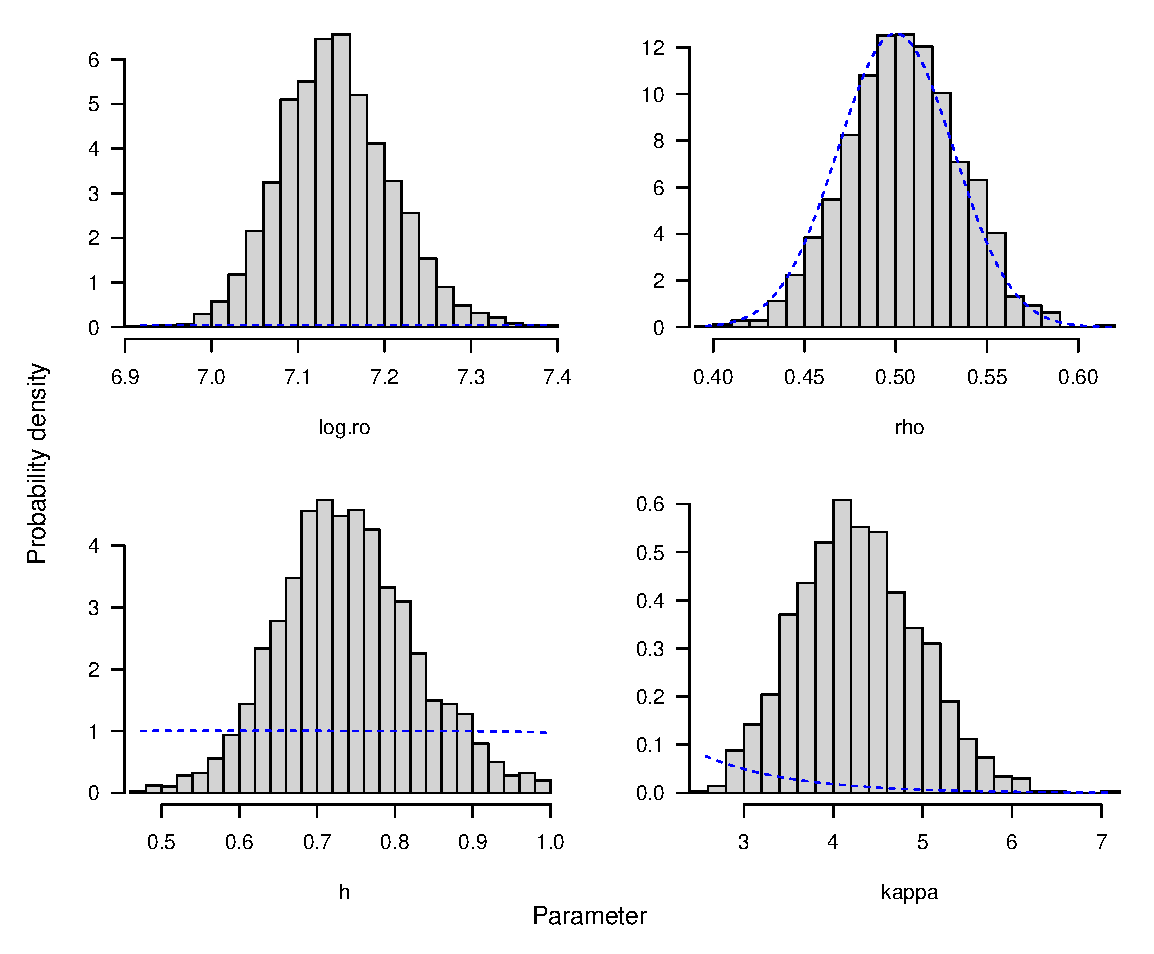
\includegraphics[width=0.9\columnwidth]{iscamFigs/nHakeparameters.pdf}\\
	\caption{Marginal posterior probability densities (histograms) and prior densities (lines) for unfished recruitment $R_0$, steepness $h$, mean recruitment $\bar{R}$ and recruitment compensation $\kappa$ for the Namibian hake case study.}\label{fig5}
\end{figurehere}

Marginal posterior densities can also be produced for derived quantities such as MSY based reference points (Fig \ref{fig6}).   Again, although not directly comparable due to structural differences between \iscam\ and the LRGS model, the marginal posterior distributions for MSY and $B_0$ are very similar.  More importantly however is that these marginal distributions can also be used to calculate the probability that the stock is currently overfished and if overfishing is occurring.  This is normally represented from a maximum likelihood perspective where the trends in biomass relative to \bmsy and fishing mortality rates relative to \fmsy are plotted against each other (these are known as KOBE plots, Fig \ref{fig7}).

\begin{figurehere}
	% Requires \usepackage{graphicx}
	\centering
	% \psfrag{bo}[c][][0.75]{$B_0$}
	% 	\psfrag{bmsy}[c][][0.75]{\bmsy}
	% 	\psfrag{msy}[c][][0.75]{MSY}
	% 	\psfrag{fmsy}[c][][0.75]{\fmsy}
	%%\includegraphics[width=\columnwidth]{iscamFigs/fig6.eps}\\
	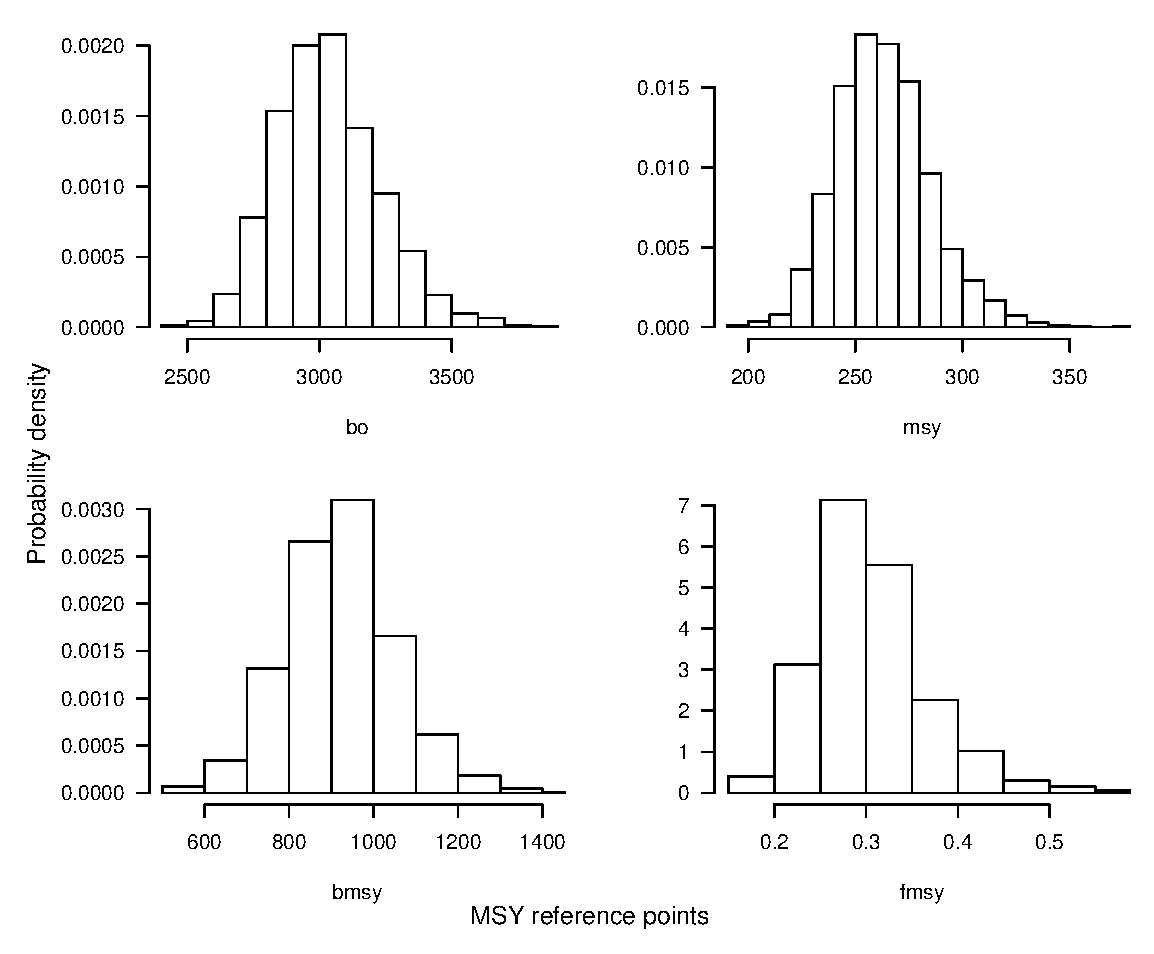
\includegraphics[width=0.9\columnwidth]{iscamFigs/nHakerefpoints.pdf}\\
	\caption{Marginal posterior probability densities for unfished spawning biomass $B_0$, optimal spawning biomass \bmsy, MSY and \fmsy\ for the Namibian hake case study.}\label{fig6}
\end{figurehere}

To represent changes in stock status over time, the default plot compares estimates of spawning stock biomass relative to the estimates of \bmsy versus fishing mortality rates relative to \fmsy.  Uncertainty in stock status for the last year is based on the joint posterior distribution and a credible interval is given by a contour plot that represents a `fried egg'.

\begin{figurehere}
	\centering
	% \psfrag{bstatus}[c][][0.75]{$B_t/$\bmsy}
	% 	\psfrag{fstatus}[c][][0.75]{$F_t/$\fmsy}
	%%\includegraphics[width=\columnwidth]{iscamFigs/fig7.eps}\\
	\includegraphics[width=0.9\columnwidth]{iscamFigs/NhakeKobeplot.pdf}\\
	\caption{Stock status plot (or Kobe plot) where the ``fried egg'' represents uncertainty.}\label{fig7}
\end{figurehere}

\end{multicols}



%%%%%%%%%%%%%%%%%%%%%%%%%%%%%%%%%%%%%%%%%%%%%%%%%%%%
%%%%%%%%%%%%%%%%%%%%%%%%%%%%%%%%%%%%%%%%%%%%%%%%%%%%
%%%%%%%%%%%%%%%%%%%%%%%%%%%%%%%%%%%%%%%%%%%%%%%%%%%%
\section{Example Assessment: the Pacific hake fishery}
\begin{multicols}{2}
\subsection{Data \& assumptions}
As more complex example assessment, the data from the Pacific hake fishery is used.  Pacific hake (\textit{Merluccius productus})  in the Northeast Pacific has a migratory coastal stock that is harvested by US and Canadian fishing fleets during the summer and late fall.  This data is an extension to the previous work in \cite{Martell2008pam}.  In this example the data has been restricted to the years 1977-2009, as this was a period when catch-age data from both the Canadian and US fisheries was available and could be aggregated using a weighted average based on the catch proportion from each nation.

The data from this fishery consists of a combined total catch, a relative abundance index from an acoustic survey conducted on a triannual and biannual basis, age-composition data from the commercial fishery, and finally age-composition data from the acoustic trawl survey. The coastal Pacific hake stock undergo an annual migration from spawning grounds in the south near Baja California Sur in the winter to summer feeding grounds to the north; the extent of the northward migration is highly variable and ranges from Oregon--Washington to Southeast Alaska in some years.  Larger/older fish tend to migrate further north.  Inter-annual variation in the extent of the migration leads to variation in selectivity to the fishery.  To accommodate the time-varying selectivity, a total of 85 nodes for a bicubic spline are estimated (17 nodes for the year effect, and 5 nodes for the age effect, see Fig. \ref{Fig3}).

\begin{figurehere}
	\centering
	\includegraphics[width=0.8\columnwidth]{iscamFigs/phakefig15.eps}\\
	\caption{Combined observed landing from the US and CAN fisheries for Pacific hake between 1977 and 2009.}\label{fig8}
\end{figurehere}

In this example it was assumed that recruitment follows a Beverton-Holt relationship, the stock is not at its unfished state in 1977, natural mortality is independent of age and constant over time, and survey selectivity is asymptotic and time-invariant.  


Here is the \iscam\ control file for the Pacific hake data, and the data file is provided at the end of this section on page \pageref{HakeDataFile}.  The observed combined landings from both the US and Canadian zones have averaged about 233,000 metric tons between 1977 and 2009, and in the last 10 years has averaged 270,000 mt with a peak in 1994 of 361,000 mt  (Fig. \ref{fig8}.)\\
\tiny
\noindent \hrulefill
\begin{alltt}
\input{../../../examples/PacificHake/Data/2010/PHake2010.ctl}
\end{alltt}
\hrulefill
\normalsize


%
%\begin{figurehere}
%	\centering
%	\includegraphics[width=0.4\columnwidth]{iscamFigs/phakefig1.eps}\\
%	\caption{Assumed age-schedule information for this example assessment.}\label{fig8b}
%\end{figurehere}


\subsection{Maximum likelihood estimates}
A total of 176 model parameters were estimated and it took  roughly 10 seconds to obtain maximum likelihood estimates, including the calculations for the Hessian matrix on a MacBook Pro, with a 2.66 GHz Intel Core i7 processor.

Maximum likelihood estimates of total biomass and spawning biomass along with estimates of $B_0$ and \bmsy are shown in Fig. \ref{fig9}.  Starting in 1977, estimates of spawning biomass was just slightly less than the estimate of \bmsy.  Starting in the 1980's, spawning biomass increased to a maximum in 1990 owing to two very large year classes (1980 and 1984, Fig. \ref{fig10}). Between 1985 and 1999, recruitment ranged between average and median values and the spawning stock biomass declined to less than \bmsy values in 2001 while fisheries removals exceeded 200,000 mt per year.  Another significant year class (1999) was responsible for rebuilding the spawning stock biomass up to 2004, and since 2005, the spawning stock biomass has continued to decline.

Information to estimate age-1 recruitment for Pacific hake comes from the catch-age composition data.  Between 1978 and 2009 the average age-1 recruitment is estimated to be 2.72 billion individuals and the median value is 1.16 billion individuals (Fig. \ref{fig11}).  The maximum likelihood estimate of the standard deviation in recruitment ($\tau$, see eq. \ref{T4.2} on page \pageref{tab:statistical_catch_age_model}) was 1.29 given the prior information specified in the control file for this assessment.


\begin{figurehere}
	\centering
	\includegraphics[width=0.9\columnwidth]{iscamFigs/phakefig2.eps}\\
	\caption{Maximum likelihood estimates of total biomass and spawning stock biomass for Pacific hake along with reference points (dotted lines) for unfished spawning biomass $B_0$ and \bmsy.}\label{fig9}
\end{figurehere}


\begin{figurehere}
	\centering
	\includegraphics[width=0.9\columnwidth]{iscamFigs/phakefig14.eps}\\
	\caption{Maximum likelihood estimates of age-1 recruits from 1978 to 2009, with median and average values shown as the horizontal dashed and dotted lines.}\label{fig10}
\end{figurehere}

Current estimates of stock status relative to \bmsy\ and the removal rate relative to \fmsy is estimated to be in the critical zone in term of the Department of Fisheries and Oceans Canada, Fisheries Management Framework (Fig. \ref{fig11}).  Estimates of the spawning stock biomass are less than 80\% of \bmsy and are currently in the cautious zone.  Estimates of fishing mortality rate are roughly 1.5 times the estimate of \fmsy.  Maximum likelihood estimates of \bmsy and \fmsy are 1.13 million mt 0.336, respectively. 

\begin{figurehere}
	\centering
	\includegraphics[width=0.9\columnwidth]{iscamFigs/phakefig8.eps}\\
	\caption{Maximum likelihood estimates of stock status ($B_t/$\bmsy) and removal rate ($F_t/$\fmsy) for Pacific hake relative to the Department of Fisheries and Oceans Canada's  Fisheries Management Framework.}\label{fig11}
\end{figurehere}

Model fit can be partially judged by the residual patterns between the observed and predicted data (Fig. \ref{fig12}).  The catch data are assumed to be measured fairly accurately with a small standard deviation ($\sigma_C=0.025$) in measurement errors; the largest residual in the catch is just less than 100 mt in 1981.  

Recall that \iscam\ directly estimates annual recruitment values, and the reported residuals in Fig. \ref{fig12} correspond to the log differences between the estimated recruitment and a Beverton-Holt model prediction where $R_0$ and steepness $h$ are the estimated parameters for the stock recruitment model.  The strong 1980, 1984 and 1999 cohorts, show up as strong positive residuals in 1981, 1985 and 2000 in the residual plot (note that the age-at-recruitment is 1 year).  The 2002 and 2004 cohorts appear to be well below the median values in recent years, and the 2005 cohort is currently estimated to be the next largest cohort since 1999.

\begin{figurehere}
	\centering
	\includegraphics[width=0.9\columnwidth]{iscamFigs/phakefig11.eps}\\
	\caption{Residuals between the observed and predicted catch, deviations between estimated recruitment and a deterministic Beverton-Holt model, and the observed and predicted relative abundance data from the acoustic survey.}\label{fig12}
\end{figurehere}


\subsection{Time-varying selectivity}
Estimates of time-varying selectivity for the commercial fishery were based on estimating 85 nodes (17 years and 5 ages) and interpolating between these nodes using a bicubic spline.  The estimated nodes in \iscam\ are equidistant, and the total number of estimated nodes is specified in the control file.  Increasing the number of estimated nodes should improve the overall fit to the age-composition data; however, this comes at the expense of increasing the associated uncertainty in overall model parameter estimates.  To ensure that the model is not over-fitting the data, there are two additional penalties that are added to the objective function that limit the rate of change in age-effects (penalty weight for second differences), and how much dome-shaped is allowed in the age-effects.  Increasing the penalty weight on second differences insures a smoothed increase or decrease in the selectivity-at-age, and increasing the weight on the dome-shaped penalty reduces the amount of dome-shaped selectivity that can occur.  Again, these penalty weights are specified in the control file  in the selectivity parameters section.

In the Pacific hake example, estimates of selectivity increase with age during the late 1970s and early 1980s (Fig. \ref{fig13}).  As the 1980 and 1984 cohorts recruit to the fishery, the selectivity shifts to younger ages, and becomes more dome-shaped.  At the peak of the spawning stock biomass in 1990, selectivity increases continuously with age, and is more or less asymptotic until the 1999 cohort enters the fishery.  Recent estimates of selectivity indicate that the 1999 cohort (age-10 in the year 2009) is still strongly selected for, but as the biomass of the 1999 cohort erodes there is an apparent increase in selectivity for older ages (Fig. \ref{fig13}).

\begin{figurehere}
	\centering
	\includegraphics[width=0.9\columnwidth]{iscamFigs/phakefig9a.eps}\\
	\caption{Estimates of selectivity for the commercial fishery.}\label{fig13}
\end{figurehere}


\begin{figurehere}
	\centering
	\includegraphics[width=0.9\columnwidth]{iscamFigs/phakefig13a.eps}\\
	\caption{Observed age-composition (top panel) and Pearson residuals between observed and predicted proportions-at-age in the commercial fishery (bottom panel, with negative residuals given by dark circles).}\label{fig13a}
\end{figurehere}

The residual patterns in the age composition data from the commercial fishery don't appear to have any significant pattern that would indicate a major model mis-specification (Fig. \ref{fig13a}).  There is a tendency for age-2 proportions to have more negative residuals and age-3 positive residuals, but over all these residuals are fairly small.  This is not much of a surprise given the flexibility of the time-varying selectivity that was assumed in the commercial fishery.


Although not shown here, the residual pattern for the survey age composition also appears to be random, and in this case a time-invariant asymptotic selectivity curve was used for the acoustic survey. Survey data from 1995 to 2007 were assumed to be twice as accurate in comparison to the data collected prior to 1995 when spatial coverage of the survey was incomplete.  Also, the 2009 survey carries no weight as this survey was contaminated by the presence of Humboldt squid (\textit{Dosidicus gigas}) during the 2009 survey.  Additional details about the data for the Pacific hake assessment and the methods used to aggregate the age-composition for the US and CAN fisheries can be found in \cite{Martell2009}.

\subsection{Bayesian implementation}
To obtain samples from the joint posterior distribution and obtain median values and credible intervals, \iscam\ was run using the Metropolis-Hastings routine that is built into ADMB.  In this example, 2000 systematic samples from a chain of length 1,000,000 was used.  The total runtime for conducting a MCMC sample  of length 1,000,000 was 39 minutes and 56 seconds with 176 estimated parameters.

The marginal posterior distributions and the corresponding prior distributions are shown in Fig. \ref{fig14}.  There is no information in the data about the underlying steepness of the stock recruitment relationship; this is clearly shown by the marginal posterior distribution for $h$ reflects the assumed (\emph{ad hoc}) prior distribution.

\begin{figurehere}
	\centering
	% \psfrag{log.ro}[c][][0.5]{$\ln(R_0)$}
	% \psfrag{log.rbar}[c][][0.5]{$\ln(\bar{R})$}
	% \psfrag{h}[c][][0.5]{$h$}
	% \psfrag{rho}[c][][0.5]{$\rho$}
	% \psfrag{log.m}[c][][0.5]{$\ln(M)$}
	% \psfrag{kappa}[c][][0.5]{$\vartheta$}
	\includegraphics[width=0.9\columnwidth]{iscamFigs/phakefig5.eps}\\
	\caption{Marginal posterior densities and prior densities for the leading parameters in \iscam.}\label{fig14}
\end{figurehere}

The prior distributions for each of the estimated leading parameters are specified in the control file.  In this example, a normal prior was assumed for the unfished recruitment ($\ln(R_0)$) and the log of the natural mortality rate ($\ln(M)$), a beta prior for the steepness ($h$) and the fraction of the total error that is associated with observation error ($\rho$), and a non-informative gamma prior for the total precision ($\vartheta$).  A uniform prior was specified for the average recruitment ($\ln(\bar{R})$).

Recent trends in the spawning stock biomass, and depletion, along with the associated uncertainty in the form of a credible interval are given in Table \ref{iscam.T1}.  Projected estimates of spawning stock depletion at the start of 2010 is 22\%, with a lower bound of 7.5\% and an upper bound of 53.2\%.  This translates into a projected spawning stock biomass of 670,000 mt with a 95\% credible interval of 255,000 mt to 1,506,000 mt.

\begin{tiny}
% latex.default(tail(t1, 10), file = filename, rowname = NULL,      caption = cap, cgroup = cgrp, n.cgroup = ncgrp, label = "iscam.T1") 
%
\begin{table}[!tbp]
 \caption{Recent trends in median estimate and 2.5\% and 97.5\% 
					credible intervals for spawning stock biomass, and
					spawning stock depletion. These estimates are based 
					on sampling the joint posterior distribution using MCMC.\label{iscam.T1}} 
 \begin{center}
 \begin{tabular}{rcrrrcrrr}\hline\hline
\multicolumn{1}{c}{\bfseries  }&
\multicolumn{1}{c}{\bfseries }&
\multicolumn{3}{c}{\bfseries Spawning stock biomass}&
\multicolumn{1}{c}{\bfseries }&
\multicolumn{3}{c}{\bfseries Depletion}
\tabularnewline \cline{1-9}
\multicolumn{1}{c}{Year}&\multicolumn{1}{c}{}&\multicolumn{1}{c}{2.5\%}&\multicolumn{1}{c}{median}&\multicolumn{1}{c}{97.5\%}&\multicolumn{1}{c}{}&\multicolumn{1}{c}{2.5\%}&\multicolumn{1}{c}{median}&\multicolumn{1}{c}{97.5\%}\tabularnewline
\hline
$2001$&&$0.877$&$1.012$&$1.226$&&$0.125$&$0.264$&$0.468$\tabularnewline
$2002$&&$1.043$&$1.217$&$1.554$&&$0.147$&$0.319$&$0.571$\tabularnewline
$2003$&&$1.874$&$2.200$&$2.945$&&$0.270$&$0.578$&$1.058$\tabularnewline
$2004$&&$2.017$&$2.395$&$3.306$&&$0.290$&$0.629$&$1.169$\tabularnewline
$2005$&&$1.692$&$2.048$&$2.976$&&$0.249$&$0.537$&$1.024$\tabularnewline
$2006$&&$1.242$&$1.569$&$2.450$&&$0.187$&$0.414$&$0.803$\tabularnewline
$2007$&&$0.851$&$1.174$&$2.053$&&$0.137$&$0.309$&$0.630$\tabularnewline
$2008$&&$0.543$&$0.886$&$1.815$&&$0.096$&$0.234$&$0.537$\tabularnewline
$2009$&&$0.312$&$0.780$&$2.099$&&$0.061$&$0.200$&$0.593$\tabularnewline
$2010$&&$0.169$&$0.726$&$2.280$&&$0.036$&$0.188$&$0.637$\tabularnewline
\hline
\end{tabular}

\end{center}

\end{table}


\end{tiny}

Relative to the spawning stock depletion reference points, the median estimate of spawning stock biomass falls in the critical zone (Fig. \ref{fig16}).  Estimates of spawn stock depletion is very uncertain; there is a fairly high probability that the stock is also in the critical zone, or less than 40\% of \bmsy.

\begin{figurehere}
	\centering
	\includegraphics[width=0.9\columnwidth]{iscamFigs/phakefig12.eps}\\
	\caption{Median estimates of spawning stock depletion and 95\% credible interval based 2000 samples from the joint posterior distribution. Transition between the critical, cautious and healthy zones is defined as 0.4\bmsy/$B_0$ and 0.8\bmsy/$B_0$, respectively }\label{fig16}
\end{figurehere}

\begin{scriptsize}
% latex.default(t1, "", file = filename, caption = cap, label = "iscam.T2") 
%
\begin{tablehere}
 \caption{Maximum likelihood estimates (MLE) and standard deviations (SD)
				based on the inverse Hessian for the six leading parameters. Median
				values and the 95\% credible interval based on posterior samples.\label{iscam.T2}} 
 \begin{center}
 \begin{tabular}{lrrrrr}\hline\hline
\multicolumn{1}{l}{}&\multicolumn{1}{c}{MLE}&\multicolumn{1}{c}{SD}&\multicolumn{1}{c}{Median}&\multicolumn{1}{c}{2.5\%}&\multicolumn{1}{c}{97.5\%}\tabularnewline
\hline
$\ln(R_0)$&$ 1.167$&$0.326$&$ 1.238$&$ 0.674$&$ 1.958$\tabularnewline
$h$&$ 0.688$&$0.214$&$ 0.669$&$ 0.370$&$ 0.932$\tabularnewline
$\ln(M)$&$-1.478$&$0.049$&$-1.457$&$-1.554$&$-1.363$\tabularnewline
$\ln(\bar{R})$&$-0.168$&$0.119$&$-0.103$&$-0.343$&$ 0.177$\tabularnewline
$\rho$&$ 0.293$&$0.043$&$ 0.305$&$ 0.227$&$ 0.405$\tabularnewline
$\vartheta$&$ 0.525$&$0.053$&$ 0.517$&$ 0.422$&$ 0.623$\tabularnewline
\hline
\end{tabular}

\end{center}

\end{tablehere}


\end{scriptsize}

\end{multicols}




Here is the data file for \iscam.
\tiny
\begin{alltt}
  \input{../../../examples/PacificHake/DATA/2010/PHake2010.dat}\label{HakeDataFile}
\end{alltt}
\normalsize

